\documentclass[]{article}

\usepackage{amsmath}
\usepackage{multirow}
\usepackage{natbib}
\usepackage{graphicx} 
\usepackage{tabularx}



\begin{document}

\title{Thermochemical Screening of Metal-Oxide Carbonation via Stoichiometric Parsing and Stability Constraints}

\author{Denario}
\date{Anthropic, Gemini \& OpenAI servers. Planet Earth.}

\maketitle
\begin{abstract}
The development of solid sorbents for industrial CO₂ capture is hindered by the conflicting requirements of strong chemical affinity for capture, low-energy thermal regeneration, and long-term structural durability. To identify materials that resolve these trade-offs, we present a high-throughput computational screening using the Materials Project database, systematically identifying 889 unique metal oxide-carbonate reaction pairs filtered for thermodynamic accessibility. Each candidate was evaluated against a comprehensive set of performance metrics, including Gibbs free energy to assess thermodynamic reversibility, volumetric expansion to predict mechanical integrity, and Tamman temperature to estimate sintering resistance. Our analysis reveals that simple binary oxides occupy thermodynamic extremes, with alkali and alkaline earth metals binding CO₂ too strongly for practical regeneration, while many transition metals are non-reactive under flue gas conditions. Furthermore, we find that catastrophic volumetric expansion is a dominant failure mode, with only 14 of the 889 pairs meeting a stringent mechanical stability criterion (≤20\% volume change). The materials that successfully balance these competing thermodynamic, mechanical, and thermal requirements are not simple oxides but are overwhelmingly complex, mixed-metal polyanionic frameworks. Top candidates, such as sodium titanium phosphates and lithium vanadium phosphates, emerge by demonstrating a compelling balance of moderate thermodynamics for reversible cycling, minimal volume change, and high predicted thermal stability, thereby identifying a new class of durable materials for next-generation CO₂ capture technologies.
\end{abstract}








\section{Introduction}
\label{sec:intro}
The development of large-scale carbon capture technologies is critical for mitigating the impact of anthropogenic CO₂ emissions from industrial point sources. Solid sorbents offer a promising pathway for capturing CO₂ from flue gas streams, but their practical implementation hinges on satisfying a set of demanding and often conflicting material properties. An ideal sorbent must not only exhibit a strong chemical affinity for CO₂ but also release it with a minimal energy penalty during thermal regeneration. Furthermore, to be economically viable, the material must maintain its structural and chemical integrity over thousands of high-temperature capture-and-release cycles.

The central challenge in sorbent design lies in navigating the inherent trade-offs between these requirements. The thermodynamics of the carbonation reaction must be precisely tuned: materials that bind CO₂ too strongly, such as many alkali and alkaline earth oxides, require excessively high regeneration temperatures, rendering the process energetically inefficient. Conversely, materials with weak CO₂ binding may be unreactive under typical flue gas conditions. Beyond this thermodynamic dilemma, sorbents face severe degradation mechanisms. The solid-state transformation from an oxide to a carbonate is often accompanied by significant volume changes, which can induce particle fracture, loss of active surface area, and a rapid decline in performance. Simultaneously, the elevated temperatures needed for regeneration can cause sintering, where particles fuse and further diminish the material's capture capacity. The search for a single material that simultaneously resolves these competing thermodynamic, mechanical, and thermal challenges has remained a primary bottleneck.

To accelerate the discovery of durable sorbents, we present a high-throughput computational screening strategy that systematically evaluates a vast chemical space. Leveraging the Materials Project database, we computationally construct and analyze 889 unique metal oxide-carbonate reaction cycles. Our approach begins by systematically parsing chemical formulas to identify all stoichiometrically balanced reaction pairs, ensuring a consistent basis for thermodynamic comparison. We then filter this dataset to include only materials that are either on the convex hull of thermodynamic stability or close to it, focusing the search on experimentally accessible compounds. Each candidate is subsequently assessed against a multi-faceted set of performance metrics designed to address the key failure modes. The Gibbs free energy of the carbonation reaction, $\Delta G$, is calculated to identify materials that operate within the optimal thermodynamic window for reversible cycling. The volumetric expansion upon carbonation is quantified to filter out materials susceptible to mechanical breakdown. Finally, the Tamman temperature is used as a proxy to estimate the material's resistance to sintering at operational temperatures.

This comprehensive screening reveals that simple binary oxides are generally poor candidates, as they tend to occupy thermodynamic extremes of being either too stable for regeneration or too unreactive for capture. We find that catastrophic volumetric expansion is a dominant and often overlooked failure mechanism, disqualifying a large fraction of otherwise promising materials. The materials that successfully emerge from our rigorous filtering process are not simple compounds but are overwhelmingly complex, mixed-metal polyanionic frameworks. By balancing these competing requirements, candidates such as sodium titanium phosphates and lithium vanadium phosphates are identified as a new class of durable sorbents that exhibit moderate reaction thermodynamics, minimal volume change, and high predicted thermal stability. This work provides a systematic framework for materials discovery and pinpoints a promising chemical space for the rational design of robust and efficient CO₂ capture technologies.

\section{Methods}
\label{sec:methods}
\subsection{Dataset and candidate selection}
The computational screening was performed using crystal structures and formation energies derived from the Materials Project database. To ensure that all candidate materials are either thermodynamically stable or synthetically accessible, the initial dataset was filtered to include only entries with an energy above the convex hull of stability less than or equal to 0.1 eV/atom. 

From this filtered set, we systematically identified potential carbonation reactions by stoichiometrically parsing the chemical formulas of all oxides and carbonates. A custom algorithm was developed to match oxide precursors with their corresponding carbonate products, ensuring that the metal cation stoichiometry was identical for each reaction pair. This process yielded a comprehensive set of 889 unique oxide-carbonate reaction pairs, representing the chemical space for the general carbonation reaction:
\begin{equation}
    M_xO_y + zCO_2 \rightarrow M_x(CO_3)_zO_y
\end{equation}
where $M_xO_y$ is the metal oxide sorbent and $M_x(CO_3)_zO_y$ is its carbonated form. All subsequent analyses were performed on these 889 reaction pairs.

\subsection{Thermodynamic analysis}
The thermodynamic viability of each carbonation reaction was assessed by calculating the Gibbs free energy of reaction, $\Delta G$, at standard flue gas conditions (T = 700 K, $P_{CO_2}$ = 0.15 bar). The Gibbs free energy was calculated using the fundamental thermodynamic relation:
\begin{equation}
    \Delta G(T, P) = \Delta H - T\Delta S
\end{equation}
The reaction enthalpy, $\Delta H$, was approximated using the 0 K formation energies ($\Delta E$) computed via Density Functional Theory (DFT) as provided in the Materials Project:
\begin{equation}
    \Delta H \approx \Delta E = E_{\text{carbonate}} - E_{\text{oxide}} - E_{CO_2}
\end{equation}
To maintain consistency with the DFT energy scale of the solid phases, a reference energy of -3.94 eV was used for the gas-phase $CO_2$ molecule.

The reaction entropy, $\Delta S$, was calculated as the difference between the entropies of the products and reactants. The entropy change of the solid phases, $\Delta S_{solid} = S_{carbonate} - S_{oxide}$, was approximated using the Dulong-Petit limit, which assumes a constant heat capacity at high temperatures. The entropy of gaseous $CO_2$ was taken from standard thermodynamic tables and adjusted to reflect the partial pressure of 0.15 bar at 700 K. The equilibrium temperature, $T_{eq}$, for each reaction was determined as the temperature at which $\Delta G = 0$, approximated by $T_{eq} \approx \Delta H / \Delta S$.

\subsection{Mechanical and thermal stability metrics}
To evaluate the long-term durability of the sorbents, we quantified two critical failure modes: mechanical degradation due to volume change and thermal degradation due to sintering.

The mechanical stability was assessed by calculating the percentage volumetric expansion ($\Delta V$) upon carbonation. Using the equilibrium crystal structure volumes ($V$) from the database, the expansion was defined as:
\begin{equation}
    \Delta V (\%) = \frac{V_{\text{carbonate}} - V_{\text{oxide}}}{V_{\text{oxide}}} \times 100\%
\end{equation}
This metric serves as a direct proxy for the mechanical stress induced during the solid-state transformation, with lower values indicating higher resistance to particle fracture and decrepitation.

Resistance to thermal sintering was estimated using the Tamman temperature ($T_T$), which approximates the onset of significant lattice diffusion and particle agglomeration. The Tamman temperature was calculated as half of the material's melting point, $T_T \approx 0.5 \times T_{melt}$. As experimental melting points are unavailable for many of the screened compounds, $T_{melt}$ was estimated for each oxide using an empirical regression model based on its DFT-calculated cohesive energy and the number of atoms in the unit cell. An "operating margin" was then defined as the difference between the Tamman temperature and the target operating temperature of 700 K, with a larger margin indicating greater resistance to sintering-induced degradation.

\subsection{Isostructural substitution analysis}
To derive rational design principles for tuning sorbent thermodynamics, we performed an isostructural substitution analysis. The well-characterized CaO (Fm-3m) $\rightarrow$ CaCO$_3$ (R-3c) and MgO (Fm-3m) $\rightarrow$ MgCO$_3$ (R-3c) reactions were used as structural templates. We identified all other reaction pairs in our dataset that shared these exact oxide and carbonate space groups, allowing for a direct comparison of the effect of cation substitution independent of crystallographic changes. For each substituted pair, we calculated the shift in reaction enthalpy ($\Delta H_{shift}$) and equilibrium temperature ($T_{eq}$) relative to the benchmark system to quantify the thermodynamic impact of altering the primary metal cation.

\subsection{Composite scoring and candidate ranking}
To identify the most promising overall candidates, a composite performance score was calculated for each of the 889 reaction pairs. This score integrated the three primary performance metrics: thermodynamic reversibility, mechanical stability, and thermal stability. Each metric was first normalized to a common scale. The Gibbs free energy ($\Delta G$) was normalized such that values closest to zero received the highest score. The volumetric expansion ($\Delta V$) was normalized to penalize large changes. The Tamman operating margin was normalized to reward higher values. The final composite score was an equally weighted sum of these three normalized metrics, providing a single, holistic figure of merit to rank all materials and identify top candidates that optimally balance the competing requirements for an ideal solid sorbent.

\section{Results}
\label{sec:results}
Our high-throughput screening pipeline evaluated 889 unique oxide-carbonate reaction pairs, filtered for thermodynamic stability, to identify materials that optimally balance the competing requirements for an ideal CO₂ sorbent. The analysis systematically quantified the thermodynamic driving force for capture, the mechanical strain from volume expansion, and the thermal resistance to sintering. The results reveal clear structure-property relationships and identify a new class of complex oxide materials that overcome the limitations of simple binary oxides.

\begin{figure*}[t]
    \centering
    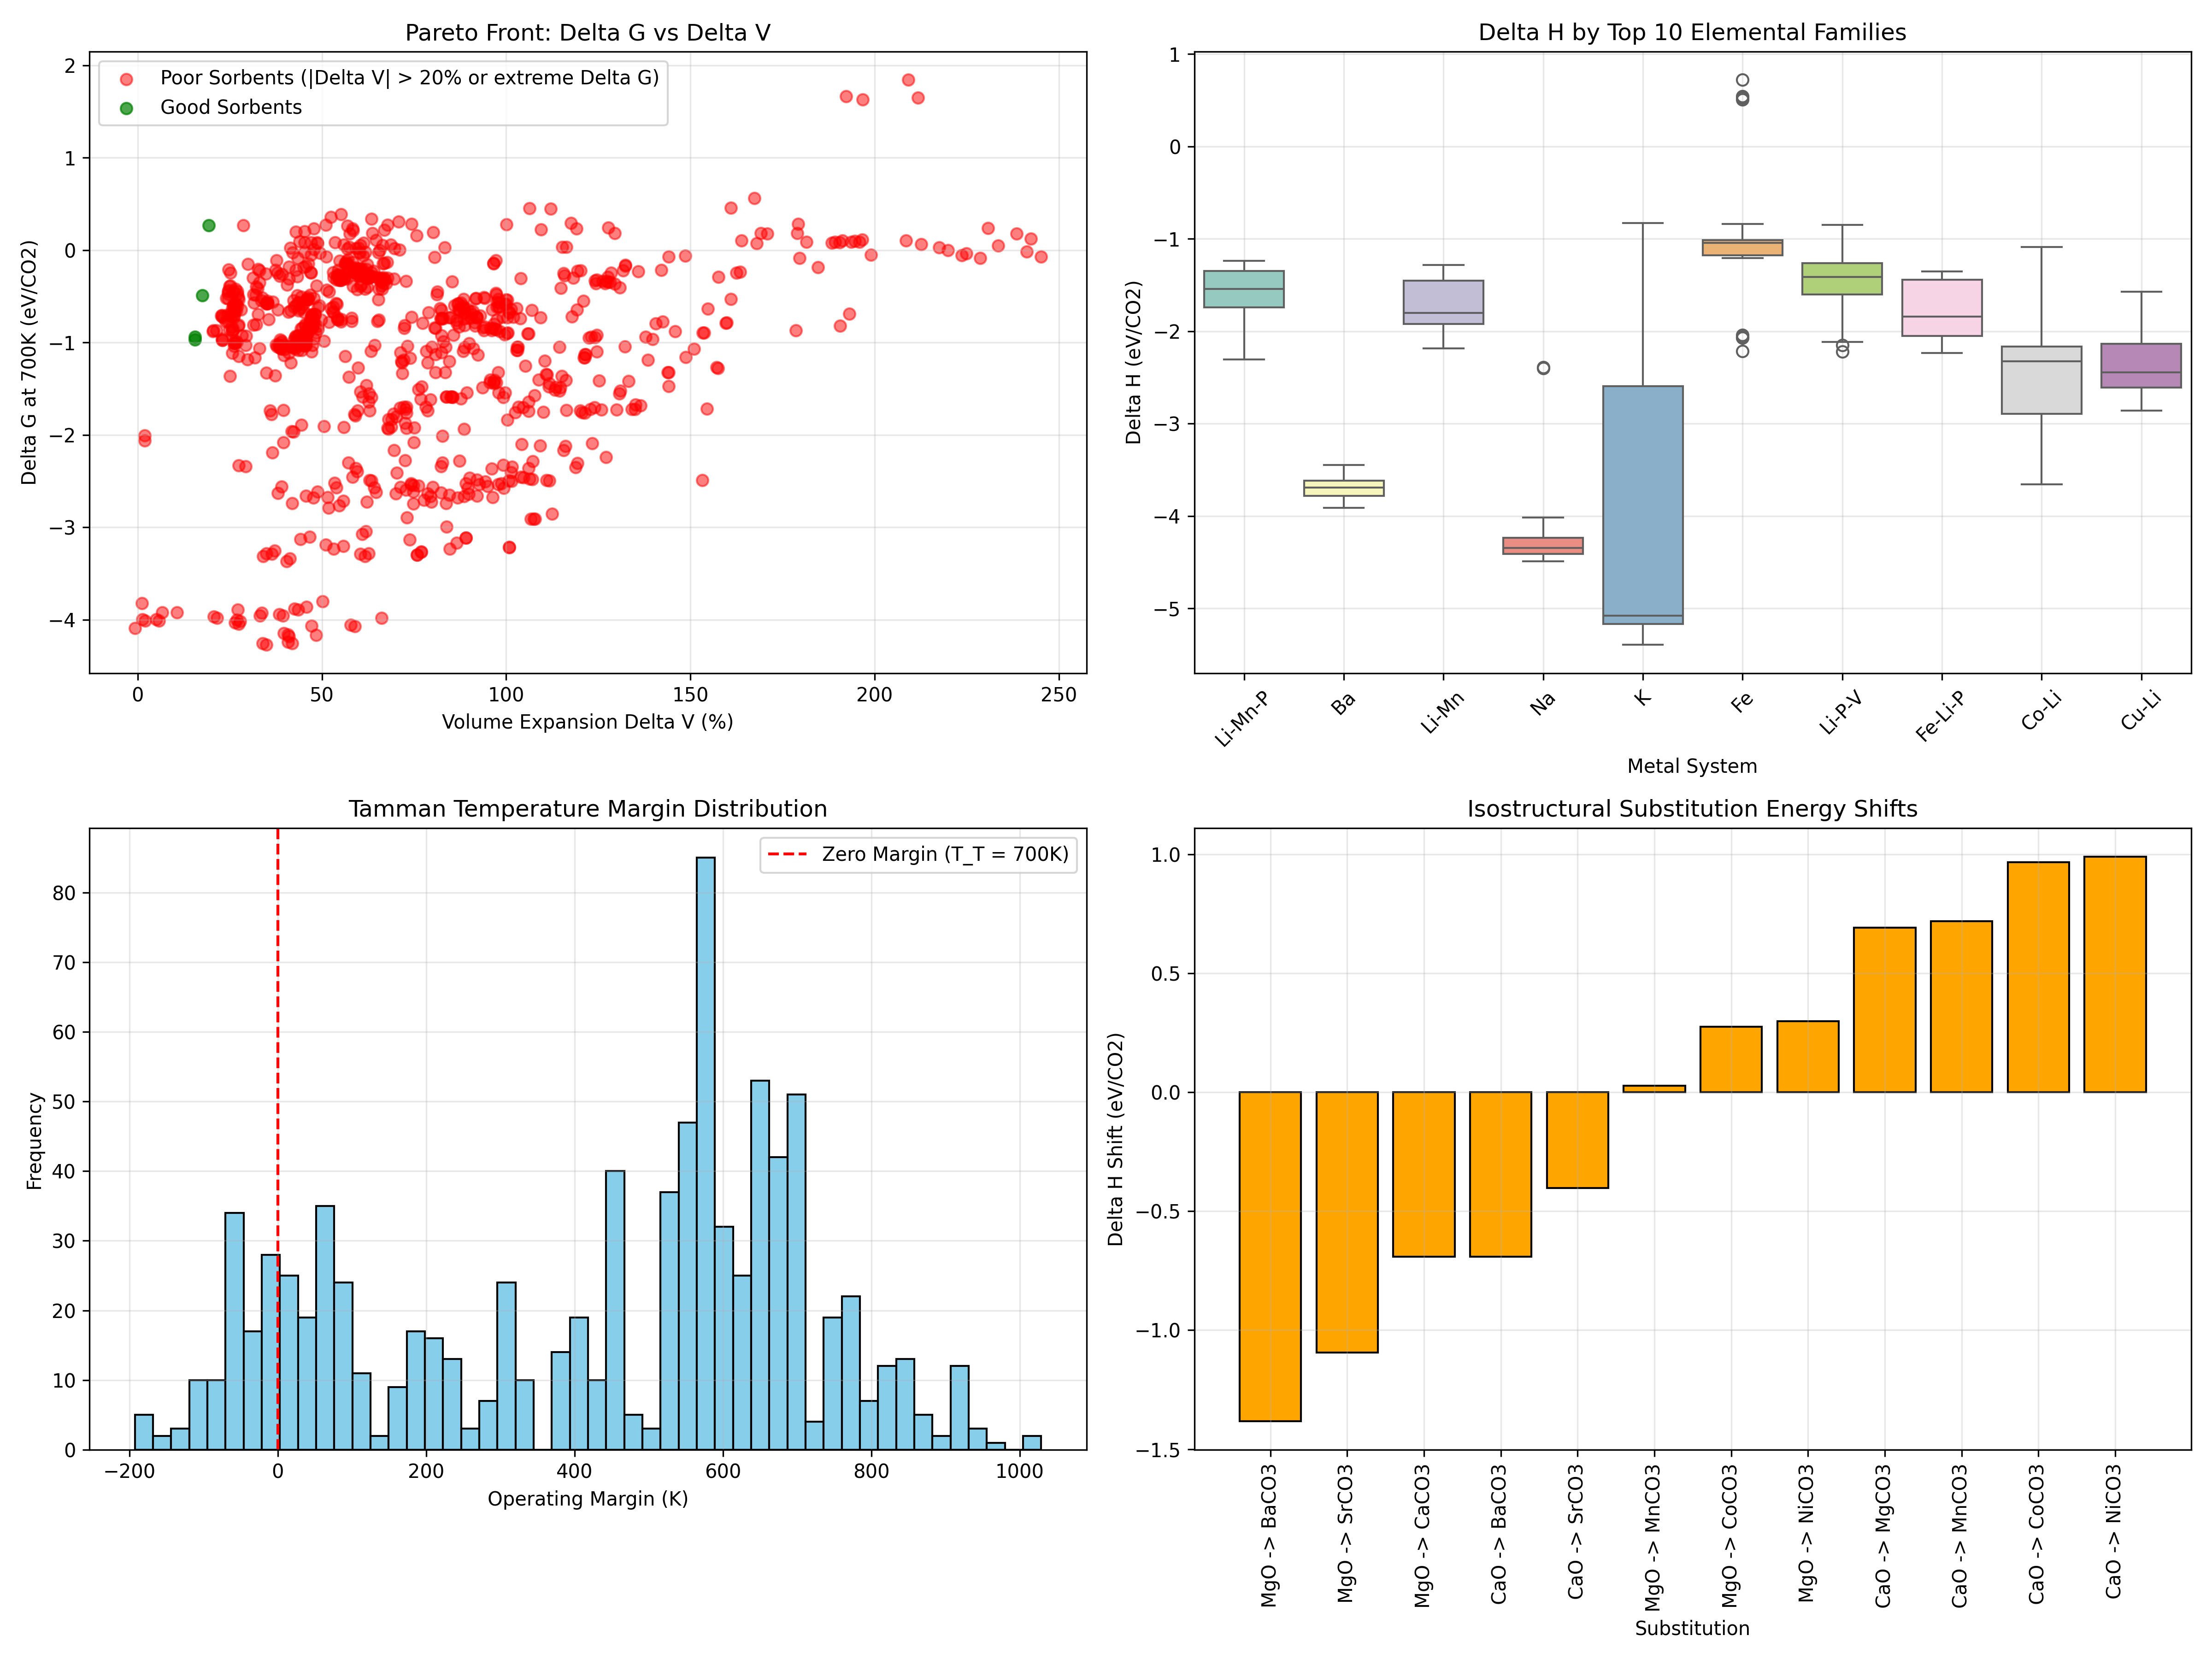
\includegraphics[width=\textwidth]{../input_files/plots/step_6_multi_panel_analysis_1_1775790796.png}
    \caption{Multifaceted screening of CO₂ sorbent properties. (Top-left) A Pareto analysis of Gibbs free energy ($\Delta$G) versus volume expansion ($\Delta$V) at 700 K demonstrates that most materials are poor sorbents due to extreme thermodynamics or catastrophic volume expansion (> 20\%), isolating a few promising candidates in the optimal region near $\Delta G = 0$ and low $\Delta V$. (Top-right) Box plots of reaction enthalpy ($\Delta$H) show that alkali and alkaline earth metals (e.g., K, Na) are highly exothermic and non-regenerable, while mixed-metal polyanionic systems (e.g., Li-P-V, Fe-Li-P) exhibit the moderate thermodynamics ideal for reversible cycling. (Bottom-left) The distribution of the Tamman temperature operating margin reveals that many candidates possess high thermal stability and resistance to sintering. (Bottom-right) Isostructural substitution analysis establishes a design rule where cation substitution systematically tunes reaction enthalpy, with less electropositive metals like Ni and Co destabilizing the carbonate and lowering the regeneration energy.}
    \label{fig:pareto_and_distributions}
\end{figure*}

\subsection{A multi-property performance landscape}
The overall performance landscape of the 889 candidates is summarized in Figure \ref{fig:pareto_and_distributions}. The Pareto plot of Gibbs free energy ($\Delta G$) versus volume expansion ($\Delta V$) at 700 K (top-left panel) immediately highlights the central challenge: most materials are unsuitable due to either extreme thermodynamics or catastrophic volume changes. The ideal sorbent must occupy the small "optimal region" near $\Delta G = 0$ eV for efficient, reversible cycling and low $\Delta V$ for mechanical stability.

The underlying thermodynamic trends are detailed in the top-right panel of Figure \ref{fig:pareto_and_distributions}. Reaction enthalpies ($\Delta H$) cluster strongly by the primary metal cation. Alkali and alkaline earth metals (e.g., K, Na, Ba) exhibit highly exothermic reactions (mean $\Delta H$ of -4.22, -4.20, and -3.69 eV/CO₂, respectively), leading to excessively stable carbonates that are non-regenerable. Conversely, many transition metal oxides, like those of iron, are non-spontaneous (mean $\Delta G$ of +0.101 eV) under flue gas conditions. The most promising materials are mixed-metal polyanionic systems (e.g., Li-P-V, Li-Mn-P), which occupy an intermediate "Goldilocks" window with mean $\Delta G$ values of -0.329 eV and -0.475 eV, respectively, ideal for reversible cycling.

Long-term durability requires resistance to thermal sintering, which we assessed using the Tamman temperature ($T_T$) operating margin ($T_T - 700$ K). The distribution in the bottom-left panel of Figure \ref{fig:pareto_and_distributions} shows that many complex oxides are highly robust. The calcium phosphate system (Ca₁₀P₆O₂₅) is a standout with a margin of 1028.9 K, while candidates like potassium titanium phosphate (KTiPO₅) also show excellent stability (margin > 950 K). This suggests that rigid polyhedral units (e.g., PO₄, TiO₆) enhance lattice cohesion and prevent thermal degradation.

To establish rational design principles, we analyzed the effect of isostructural cation substitution on reaction thermodynamics, shown in the bottom-right panel of Figure \ref{fig:pareto_and_distributions}. Using the CaO $\rightarrow$ CaCO₃ reaction as a template, we found a clear trend: substituting Ca with more electropositive metals (e.g., Sr, Ba) makes the reaction more exothermic, while substitution with less electropositive transition metals (e.g., Mn, Co, Ni) systematically destabilizes the carbonate. This provides a powerful predictive rule: the M-O bond covalency can be used to fine-tune the thermodynamics for optimal performance.

\subsection{Volumetric expansion as a critical failure mode}
A primary mechanism for the mechanical failure of solid sorbents is the stress induced by volume changes during carbonation and decarbonation cycles. Our analysis reveals this is a dominant and often disqualifying factor. Figure \ref{fig:volume_expansion} shows the distribution of molar volume expansion ($\Delta V$) for all 889 reaction pairs. The distribution is heavily right-skewed, with a mean expansion of 74.85\% and some materials expanding by over 200\%. Such large, repeated structural changes lead to particle pulverization, loss of surface area, and a rapid decline in CO₂ capture capacity.

\begin{figure}[htbp]
    \centering
    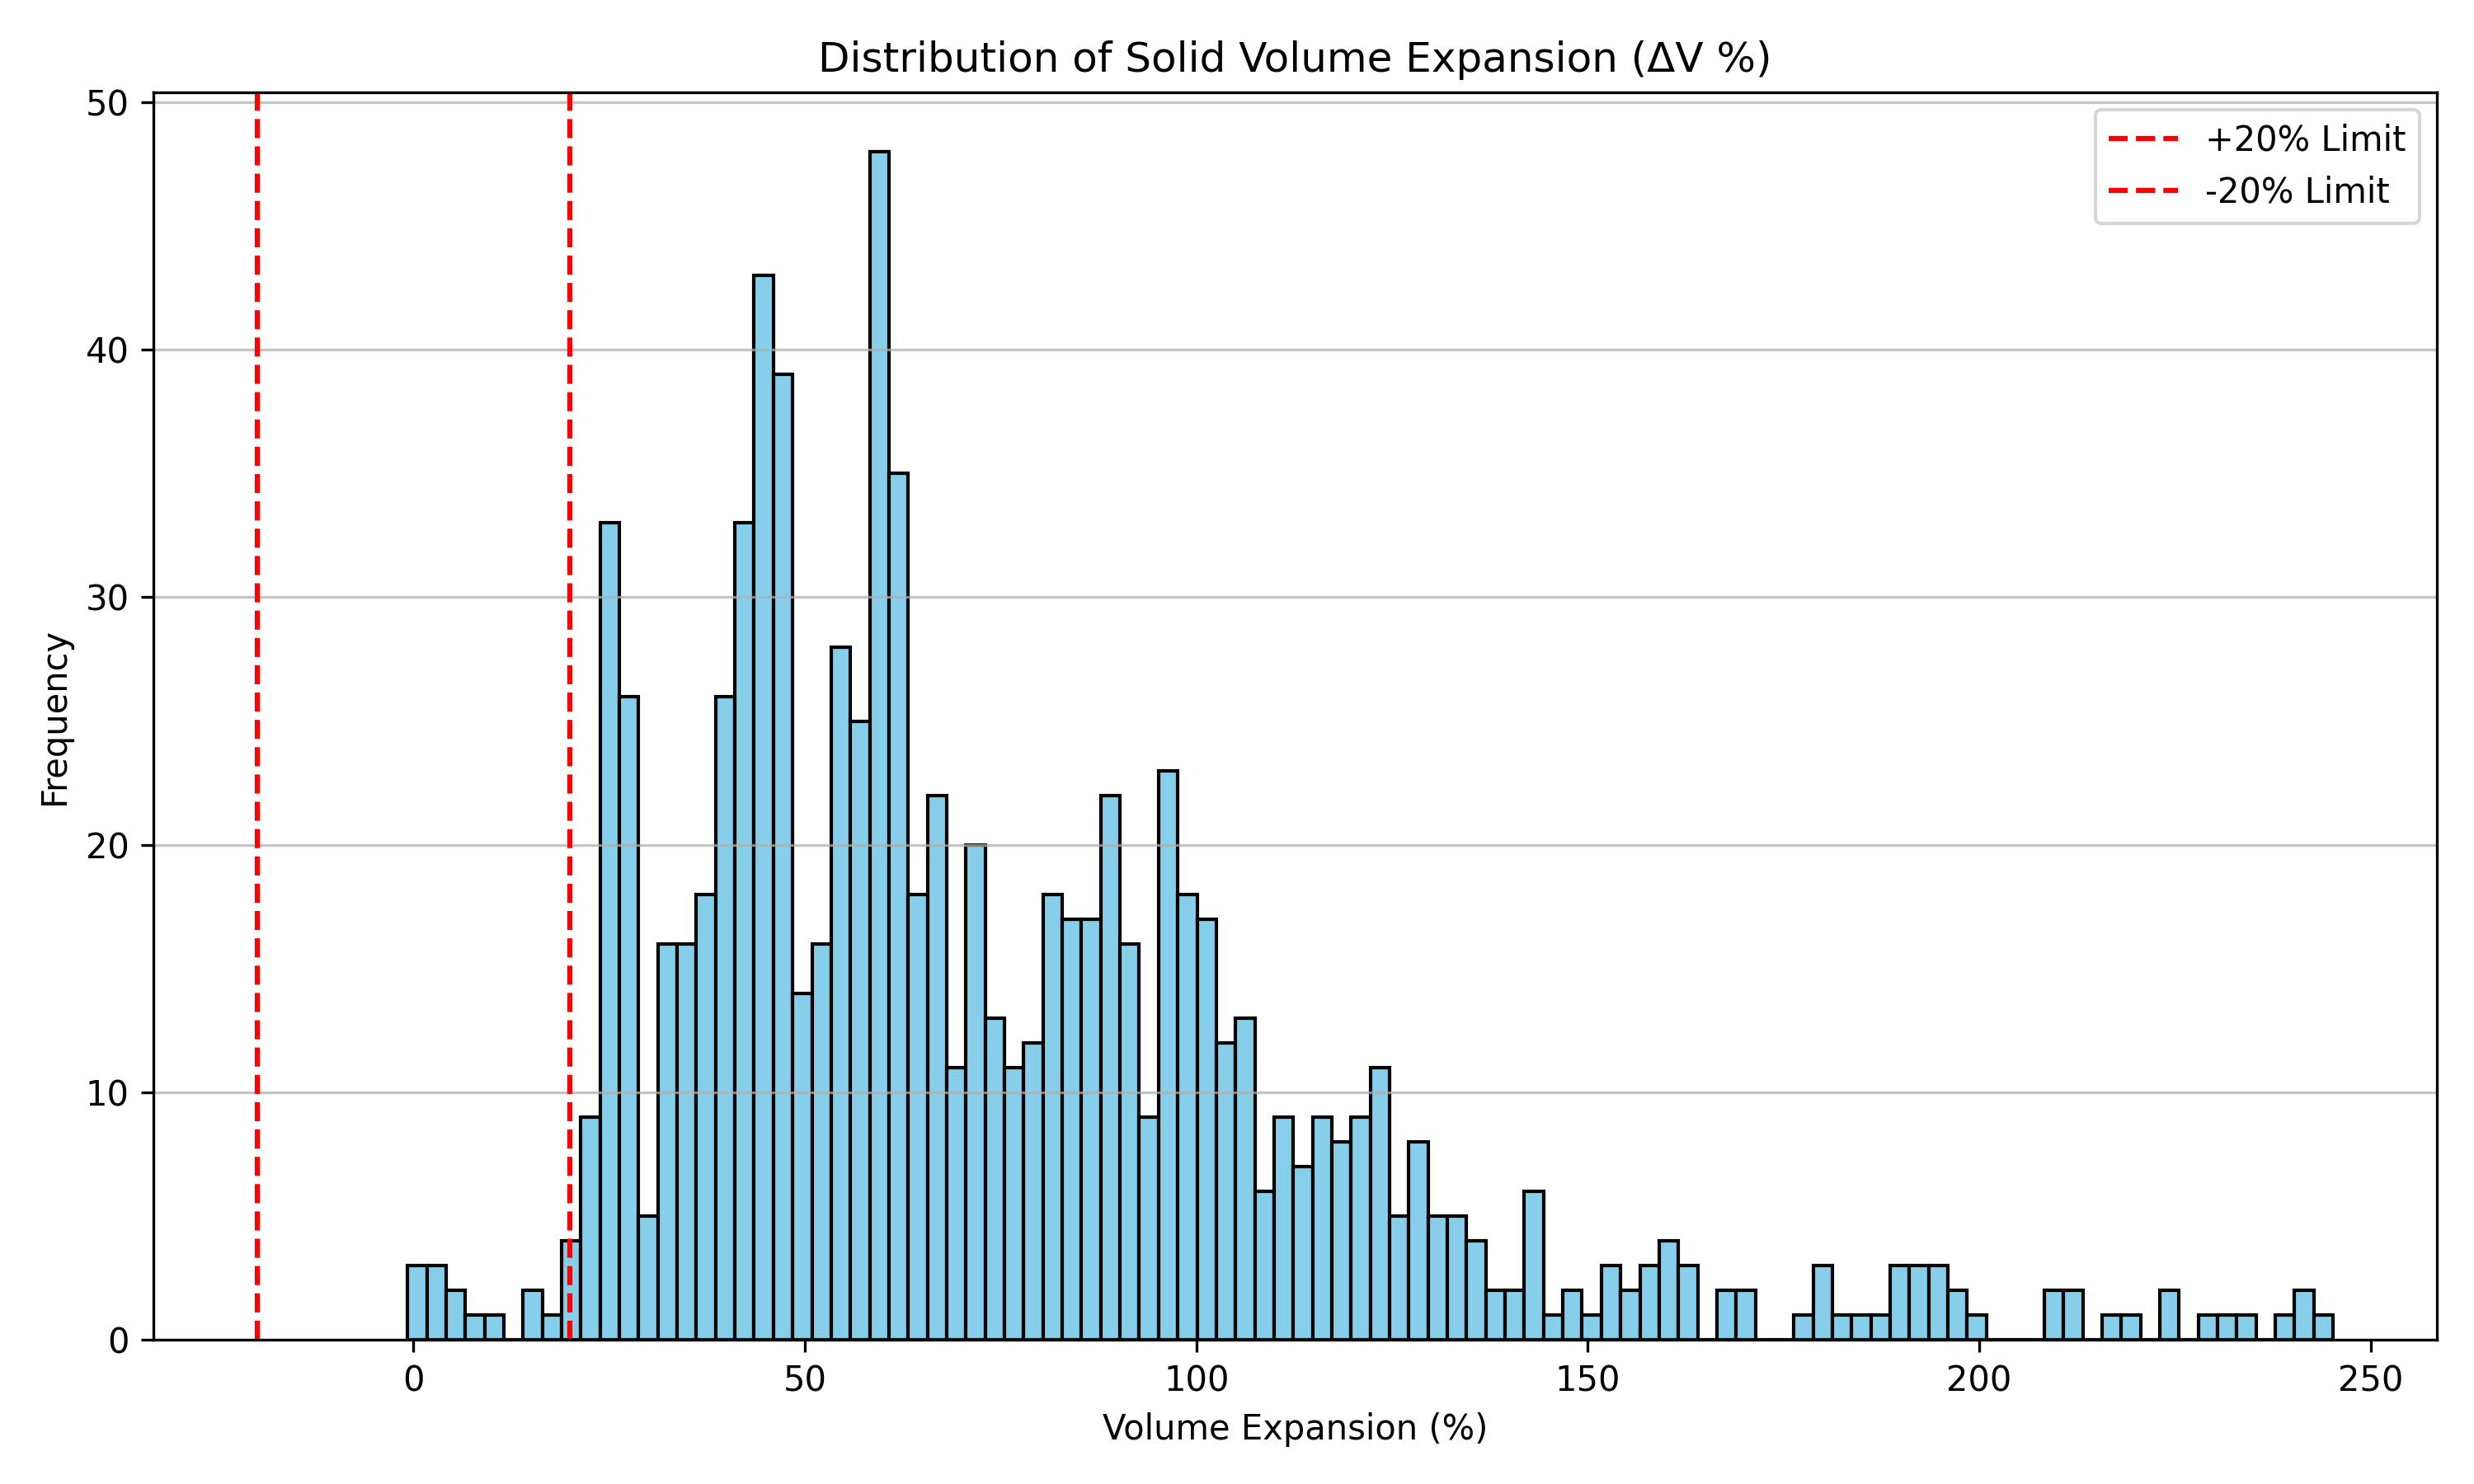
\includegraphics[width=0.5\textwidth]{../input_files/plots/step_3_volume_expansion_histogram_1775790499.png}
    \caption{Distribution of the molar volume expansion ($\Delta$V) upon carbonation for the 889 screened reaction pairs. The histogram reveals a heavily right-skewed distribution with a mean expansion of 74.85\%, indicating that most materials undergo significant structural swelling detrimental to mechanical integrity. The red dashed lines highlight the strict mechanical robustness filter applied ($|\Delta V| \leq 20\%$), visually demonstrating the rarity of dimensionally stable candidates, with only 14 reactions meeting this criterion.}
    \label{fig:volume_expansion}
\end{figure}

To identify mechanically robust candidates, we applied a stringent filter, retaining only materials with an absolute volume change of 20\% or less. As highlighted in Figure \ref{fig:volume_expansion}, this filter drastically reduces the candidate pool to just 14 reaction pairs, underscoring the rarity of dimensionally stable sorbents. This is also evident in the Pareto plot (Figure \ref{fig:pareto_and_distributions}, top-left), where the vast majority of materials lie outside the desired low-$\Delta V$ region. The materials that satisfy this criterion are predominantly complex, open-framework structures. For instance, the sodium aluminosilicate system (Na₈Al₆Si₆O₂₅) exhibits a near-zero volume change (-0.77\% to 1.17\%), as CO₂ can be accommodated within its existing microporous structure. Similarly, the calcium phosphate system (Ca₁₀P₆O₂₅) shows a minimal expansion of $\sim$1.9\%. These results pinpoint open-framework polyanionic structures as a key motif for designing mechanically durable sorbents.

\subsection{Composite ranking and promising polyanionic sorbents}
To identify the most promising candidates overall, we integrated the key performance metrics—thermodynamic reversibility ($\Delta G$), mechanical stability ($\Delta V$), and thermal durability (Tamman margin)—into a single composite score. This holistic ranking moves the focus from materials that excel in one property to those that strike an optimal balance among all three.

The top-ranked candidates are overwhelmingly complex, mixed-metal polyanionic frameworks, representing a significant departure from traditional simple oxides. The highest-scoring material is sodium titanium phosphate (NaTiPO₅), which exhibits a nearly ideal $\Delta G$ of +0.010 eV at 700 K, a moderate volume expansion of 47.8\%, and an exceptional thermal operating margin of 934.2 K. Closely following is potassium titanium phosphate (KTiPO₅), with a $\Delta G$ of -0.003 eV and a margin of 958.3 K. Other promising candidates include lithium vanadium phosphates (e.g., LiVPO₅) and silicates (e.g., Li₂VSiO₅), which also balance near-zero $\Delta G$ values with manageable volume expansions (30-45\%) and high thermal stability.

As visualized in the Pareto plot (Figure \ref{fig:pareto_and_distributions}, top-left), these top candidates occupy the coveted region of near-zero $\Delta G$ and low-to-moderate $\Delta V$. Unlike CaO, which is thermodynamically robust but requires very high regeneration temperatures and suffers from sintering, these polyanionic materials are predicted to cycle reversibly at lower temperatures while resisting both mechanical and thermal degradation. Their discovery provides a data-driven roadmap for the experimental development of a new generation of durable, high-performance solid sorbents for industrial CO₂ capture.

\section{Conclusions}
\label{sec:conclusions}
This paper addresses the central challenge in solid sorbent design for CO₂ capture: the need to simultaneously satisfy the conflicting requirements of favorable reaction thermodynamics, high mechanical durability, and robust thermal stability. To navigate these trade-offs, we developed and applied a high-throughput computational screening methodology to systematically evaluate a vast chemical space of potential sorbent materials.

Our approach began by identifying 889 unique metal oxide-carbonate reaction pairs from the Materials Project database, filtered to include only thermodynamically stable or near-stable compounds. Each candidate was then assessed against a comprehensive set of performance metrics. The Gibbs free energy of reaction was calculated to evaluate thermodynamic viability for reversible cycling under flue gas conditions. The percentage volumetric expansion upon carbonation was quantified to predict mechanical integrity. Finally, the Tamman temperature was used as a proxy to estimate the material's resistance to thermal sintering during high-temperature operation.

The screening revealed several key findings. We found that simple binary oxides are generally poor candidates, as they occupy thermodynamic extremes. Alkali and alkaline earth oxides bind CO₂ too strongly for energy-efficient regeneration, while many transition metal oxides are unreactive. Furthermore, our analysis identified catastrophic volumetric expansion as a dominant and often overlooked failure mode. The majority of materials exhibited volume changes far exceeding 20\%, a threshold for mechanical stability, with only 14 of the 889 candidates meeting this stringent criterion. This result underscores the critical importance of dimensional stability for long-term sorbent performance.

From this work, we have learned that the materials best suited to resolve these competing demands are not simple compounds but are overwhelmingly complex, mixed-metal polyanionic frameworks. Top-performing candidates, such as sodium titanium phosphate (NaTiPO₅) and lithium vanadium phosphates, emerged from our screening by demonstrating a compelling balance of all three properties: moderate thermodynamics for reversible cycling, manageable volume expansion, and high predicted thermal stability. The isostructural substitution analysis further provided a rational design principle, showing that reaction thermodynamics can be systematically tuned by altering cation chemistry. By providing a data-driven framework for materials discovery, this study pinpoints a new and promising class of polyanionic materials for the rational design of durable, next-generation solid sorbents for industrial CO₂ capture.


\bibliography{bibliography}{}
\bibliographystyle{unsrt}

\end{document}
